\chapter[Detailed Description]{Detailed Description}
\section[Mechanics of Evolution RTS]{Mechanics of Evolution RTS}
Evolution RTS \cite{EvolutionRTS} is an open source game modification created for the Spring
engine. It's a Real-Time Strategy game featuring both micro and macro-management with
intense battles, real time meaning it's not turn based and that all the players can
issue orders at any time.

The resource gathering system is automated; i.e. you construct resource gathering
buildings that collects the resources automatically, giving you a constant stream
of income. There are two different kinds of resources; energy and metal. Energy
can be produced with three different buildings: solar collector, fusion reactor
and geothermal power plant. Metal can only be produced with two buildings: metal
extractor and metal maker. The metal extractor building has to be built on top of
special sites on the map, these sites are called ``extraction points'' and are
very important for map control and metal income, since they produce much more
metal than the metal maker building. Metal is used to construct additional units
whereas energy is needed when units fire their weapons---some buildings also
consume energy that is needed for their use; shield generator is one kind of
building that always consumes energy.


To construct units the player need to have factories. There are several different kind of units in
Evolution RTS: Flying, amphibious, all-terrain\footnote{Can travel on any terrain, even over cliff
edges.}, and ground units. As a side not, Al Ice does not use any amphibious units.

\subsection[Armor System]{Armor System}
\label{sec:armor_system}
\index{armor type}
\index{damage type}
\index{armor system}
Evolution RTS uses an armor system \cite{EvolutionRTS10} that simplifies the damage calculation
between weapons and unit armor; both for balancing units, although this is not our area, and generating a priority for what
units to create which Al Ice does; see \ref{sec:priority_system} for how the priority system works.

The damage a unit will do against another unit is calculated by adding it's weapon damage times the
damage multiplier. The damage multiplier is calculated by the armor type the unit who gets hit has
and the damage type of weapon that fired against the hit unit. Each unit has a specified armor and
weapon type; provided the unit has a weapon at all. The damage multiplier chart is shown in figure
\ref{fig:damage_multiplier_chart}
\begin{figure}[tb]
\centering
\caption{Evolution RTS damage multiplier chart}
\label{fig:damage_multiplier_chart}
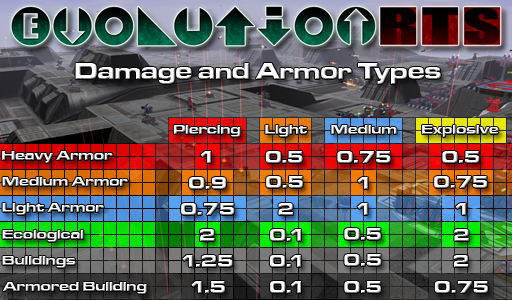
\includegraphics[width=0.9\textwidth]{evo_damage_chart}
\end{figure}

\section{Mechanics of Al Ice System}
In the following sections the most important mechanics of Al Ice are described.
Spring Interface; how the interaction and events are handled.
General; the mastermind of Al Ice.
Units; how we handle our own units.
Enemy information; how enemy information is gathered, stored, and used. 
Extraction point mapping; how we handle the extraction points on the map, i.e. which are free, under
our control, and under enemy control.
The task system; how tasks works, how they are handled, and the connection with units. In
addition to the task system the tasks that are central in Al Ice are described; the scouting tasks,
and the attack task.

\subsection{Spring Wrapper}
Details about the current game can be extracted from this. However it is only possible to get the
information that is either available from start or that the AI can see; meaning that enemy
information can only be extracted from those units that we can see at the moment. If we want to save
some information that needs to be done internally by the AI and is exactly what
\ref{sec:enemy_information} \nameref{sec:enemy_information} and \ref{sec:extraction_point_mapping}
\nameref{sec:extraction_point_mapping} does.

Available features from the start are the resource positions; i.e. where metal extraction points can
be located, how large the map is, our start position, the available units, etc.

\subsubsection{Events}
Everything of the AI is handled through events, whereas the \emph{update} is the most
notable event where a major part of Al Ice gets updated---the event sends the current frame of the
game\footnote{Spring always simulates a frame rate of 30 frames per second; meaning that the game
time can be extracted from this.}. Apart from the update event some more standard events exists;
when a unit or enemy is created, destroyed, finished, and when an enemy enters and leaves
line-of-sight. To listen to these events other agents need to implement the appropriate handler,
that has approximately the same name as the event. It should then add itself as an observer to
the Spring Wrapper and will then listen to all the events it implements.

If an agent wants to listen to a specific unit's or enemy's event it will need to implement
specific handlers for unit events or enemy events respectively. To start listening to the events the
agents should add itself as an observer for all the units it wants to listen to.

This system makes it very easy to listen to events and only to listen to those that are relevant for
the agent.

\subsection{Units}
\label{sec:units}
All the units that are available in Evolution RTS are grouped with some useful attributes by Al
Ice---these are not the units that are currently in play but units that can be built or summoned in
one way or another. It's important to note that a unit in Spring can be both a mobile unit and a
building; in fact everything that can be 'marked' is a unit, even trees.
\begin{description}
\item[unitDef] The unit's definition used by the Spring Engine.
\item[unitName] The name of the unit; not the human-readable name but the 'definition'.
\item[canAttackAir] If the unit has the ability to attack air; for simpler checking instead of
checking it's weapons.
\item[armorType] The armor type that the unit has. Can be one of the armor types shown in figure
\ref{fig:damage_multiplier_chart}
\item[damageType] The damage type that the unit has; provided that the unit has a weapon at all. Can
be one of the damage types shown in figure \ref{fig:damage_multiplier_chart}
\item[build] True if the unit should be used in the building priority; i.e. if Al Ice should use it
or not.
\item[groups] The groups that the unit belongs to. The groups are described more thoroughly in
\ref{sec:group} \nameref{sec:group}.
\end{description}
The unitName, canAttackAir, build, and groups are set in the source-code while the others values are
set during the initialization. The canAttackAir flag would ideally be set in the initialization, but
that information was rather hard to extract; therefore the
canAttackAir is now statically defined in the code.

\subsubsection{Groups}\index{groups}
\label{sec:group}
Units are grouped by their primary use; the groups are static and set in the source code. There are
currently nine groups---however, more can be added easily to the units. Most units are only in one
of the nine groups except the different builders.

\begin{description}
\item[Attack force]\index{attack force} Units belonging to the attack force are mobile units that
are able to attack. Both airborne units as ground units belong to this group.
\item[Armored building]\index{building!armored} Armored buildings consist of buildings that are
able to attack.
\item[Builder]\index{builder} All units that can build something belongs to this group. This
group is primarily used to build new builders for the unit with the highest priority, and as a
wrapper for all the different builders; if there is some information that needs to be extracted from
them. Builders should also belong to another group; \emph{factory} or \emph{mobile builders}, which is
mainly used for the priority generation. See \ref{sec:priority_system} for more information
about the priority system.
\item[Factory]\index{building!factory}\index{builder!factory|see{building-factory}} A group for
all the factories in the game; i.e. builders that are buildings. Because a factory is a builder it should also belong to the builder group.
\item[Mobile builder]\index{builder!mobile} Used for all the mobile builders in the game. As with
factories, mobile builders should also belong to the builder group.
\item[Economic]\index{building!economic} These are the units (buildings) that produces either metal
or energy.
\item[Scout]\index{scout} Units that are dedicated to scouting should be a part of this group. In
Evolution RTS there is one airborne unit which has this as it's speciality; wide line-of-sight and
because it's airborne its speed is much faster than ground units. There is also a rather fast
amphibious scout; however as Al Ice doesn't use amphibious units this scout isn't used.
\item[Utility building]\index{building!utility} Consists of all the buildings that gives the player,
in this case Al Ice, with more strategic options; like radar tower, radar-jammer, and nuclear missile silo.
This group isn't used in v0.3 of Al Ice.
\item[Healer]\index{healer} Healers are those specially assigned to heal (repair) the damaged units.
In Evolution RTS all mobile builders can heal, but only the ORBs are designated healers. This group
isn't used in v0.3 of Al Ice.
\end{description}



\subsection{Enemy Information}
\label{sec:enemy_information}
Al Ice needs to know how many enemy units there are, otherwise the priority calculation will be
ineffective. It also needs to know the positions of the enemy units to be able to order attacks. To
meet these demands Al Ice has a uses an agent 'Sighted Enemies'\index{sighted enemies} who's
job is to handle and update all enemy unit information. Since Al Ice does not cheat it would loose information about the enemy unit
if it moves out of sight. That's why the last known enemy position needs to be saved. SightedEnemies
works a lot like extraction point mapping\index{extraction point!map} and updates itself
automatically---it also updates the positions of sighted enemies regularly, since units can
change positions, which metal extraction points can't. Various information can be extracted from
Sighted Enemies; a list of all enemy units---ordered by armor and damage type if wanted, how much
armor and DPS the enemy has grouped by armor and damage type respectively, and the closest enemy to
a specified point mainly when ordering attacks.


\subsection{Extraction point mapping}
\label{sec:extraction_point_mapping}
Al Ice needs to save all the information the scouting tasks collects,
information about which extraction points are free for the taking and which points are occupied by an
enemy. To save this information the system listens to events from the Spring engine, such events as: enemy enters line
of sight, enemy destroyed, unit created and unit destroyed. This way Al Ice will automatically
update the information about an extraction point as any unit, not only a scouting unit, passes by
and saves it to a vector. The \emph{Extraction Point Map} agent has methods for calculating and
returning the position of the closest extraction point by a specified owner. This allows the
General\index{General} to expand Al Ice's resource income and to plan future attacks on enemy
outpost's.

\subsection{Priority System}
\label{sec:priority_system}
\index{priority system}
Instead of assigning priorities to task, with the exception of a task priority for a task unit
\ref{sec:task_priority}, the priorities are assigned to the available units. The system is mostly
based on other articles \cite{Dill06,Dill08} for generating priorities, grouping them, and how to
balance them in a more isolated manner.

The units available in the priority system are only those considered at the moment; usually being all
that Al Ice are specified to build---which is done statically in the code.  See \ref{sec:units} on
how the units and groups are handled. The priority system will only generate\footnote{generate and
calculate has the same meaning and are used interchangeably.} new priorities when necessary; i.e.
when there is an available builder. It checks for available builders a few times each second, thus
not making the system generating new priorities when an available builder which can't build any of
the units in the current priority list exists. 


The priorities are divided into groups; made for the simplicity of
tweaking priorities with the use of specific multipliers, minimum, and/or
maximum values for a group. How the specific group priorities are generated
is described in more detail under each group's paragraph.

When generating priorities for units, some will have no or a low priority; those under
this threshold will never make it into the priority list. This functionality is useful when building
a specific unit, or if all units from a group should be prohibited at all costs. It's currently used
with the \emph{economics only}\index{economics only} period, which is run just after the
\emph{initial build sequence}\index{initial build sequence} is completed. In this time all other groups are set to
0 in priority---this makes the available builders to only build economic buildings and boost our
income in the beginning of the game. If an available builder can't build any units in the generated priority list it is skipped.

In the first stage of the priority generation it generates the basic information about the attack
force and armored buildings priority. These are described more thoroughly in their respective
paragraph. The second stage iterates through all the units that is taken into consideration when
generating the priorities. Since all units belong to at least one group, it's then up to that group
to generate the priority for the unit. As always some units need special treatment---it's the group's
responsibility to handle the special algorithm needed for the priority generation of the unit. To
handle 'special' units the group simply checks if a unit needs any special treatment using an
if--else if--else statement which contains the units definition name. An example of this could be the
airborne builder, which is the only builder from the mobile builder group that will get another
priority than the minimum builder priority---the number of airborne builders will slowly, but
linearly, increase during the game. If the unit doesn't need any special treatment it will default
into the else statement and use the default priority generation for the group. If a unit happens to
belong to more than one group it will only keep the highest generated priority. After the priority is
generated it is either added to the priority list or discarded if the priority is too low, as
described earlier. The third and final stage consists of sorting the priority list and then adjusting
the builder priorities; described in the builder group paragraph.





\subsubsection{Group Priority Generation}
\paragraph{Attack Force}
\index{priority!attack force}
\index{attack force}
The main calculation of the attack force priority is done in the first stage of
the priority generation. The general idea is that the priorities generated are
based on what armor type is good against them; i.e. what armor type the enemy can deal least damage
to, depending on their current units, and what damage type is good against
them; i.e. what damage type our units should have that will make them destroy all the enemy
units in the least time. Only units that can do us harm will be considered into the
calculation; i.e. the enemies' attack forces and armored buildings. How the priorities are generated
are described in more detail below.

\subparagraph{Damage type priority generation}
\index{damage type}
First of all the priority for all damage types are generated. The pseudo-code
describes how the priority is generated and is described in listing
\ref{lst:attack_force_damage_priority}.
\begin{lstfloat}
\begin{lstlisting}[caption={Damage Type Priority},label={lst:attack_force_damage_priority}]
Map<String, Double> tempDamageHealth;
double maxHealth = Double.MIN_VALUE;
for (all damage types) {
	double health = 0.0;
	for (all armor types) {
		health += enemyArmorTypeHealth(armorType) / damageMultiplier(armorType, damageType);
	}
	if (health > maxHealth) {
		maxHealth = health;
	}
	tempDamageHealth.put(damageType, health);
}
\end{lstlisting}
\end{lstfloat}
The \texttt{enemyArmorTypeHealth(armorType)} returns the total seen health that
the enemies have of the specified armor type.
\texttt{damageMultiplier(armorType, damageType)} returns exactly what it says;
the damage multiplier between the specified armor and damage type. See \ref{sec:armor_system} on
how the Armor System works. The value you get from this algorithm is how much health the enemy would have had if the
DPS\footnote{Damage per second.} isn't changed depending on the armor type. E.g. if the unit has
a default health of 1000, and our damage type's effectiveness is 0.5 then it would be the same
as making the effectiveness 1.0, keeping the DPS value, and divide the health with the
effectiveness increasing the health to 2000. As can be seen this will generate higher health if
the enemy damage type is ineffective against the armor type---thus the damage type that has lowest
total health is the damage type that should be prioritized.

To keep the priority in reasonable ranges it needs to be scaled, but also inverted since the damage type with
lowest health should get the highest priority. The pseudo-code for this is
described in listing \ref{lst:attack_force_damage_scale}.
\begin{lstfloat}
\begin{lstlisting}[caption={Damage Type Priority Scaling},label={lst:attack_force_damage_scale}]
double scaleFactor = PRIORITY_MAX - PRIORITY_MIN;
for (healths in tempDamageHealth) {
	double scaledPriority = scaleFactor * health / maxHealth;
	// Invert the priority
	scaledPriority = scaleFactor - scaledPriority + PRIORITY_MIN;
	
	for (all armor types) {
		insertIntoMatrix(armorType, damageType, scaledPriority);
	}
}
\end{lstlisting}
\end{lstfloat}

First the priority, actually the health, gets scaled between 0.0 and scaleFactor. E.g. if
PRIORITY\_MAX is 20 and PRIORITY\_MIN is 10 then scaleFactor will be equal to 10. The priority is
then inverted; note, to get the highest priority (20) the health needs to be 0 thus the priorities
will be linearly scaled. Then the scaled priority is added to the matrix for all armor types. E.g.
if you think of the matrix as columns and rows the scaled priority is added column-wise for each
damage type. Then the scaled priority from the armor calculation will be multiplied in row-wise.

\subparagraph{Armor type priority generation}
\index{armor type}
It's now time to generate armor type priorities from the enemies' damage types, that is which type
of units that will withstand longest if all enemy units would target randomly on our units. The
concept is really the same as the damage type priority generation, see listing
\ref{lst:attack_force_armor_priority}. However there are some subtle differences described below.

\begin{lstfloat}
\begin{lstlisting}[caption={Armor Type Priority},label={lst:attack_force_armor_priority}]
Map<String, Double> tempArmorTypeDps;
double maxDps = Double.MIN_VALUE;
// Start with armor types instead of damage types
for (all armor types) {
	double dps = 0.0;
	for (all damage types) {
		dps += enemyDamageTypeDps(damageType) * damageMultiplier(armorType, damageType);
	}
	if (maxDps < dps) {
		maxDps = dps;
	}
	tempArmorTypeDps.put(armorType, dps);
}
\end{lstlisting}
\end{lstfloat}

The for-loops has now exchanged places; i.e. instead of \texttt{for (all damage types)} being
the outer loop the \texttt{for (all armor types)} is now the outer loop. The \texttt{dps} is how
much total DPS the enemy can do on the current armor type. Thus the armor type with the lowest DPS should be
prioritized. As with the damage type priority the value needs to be scaled and inverted. The
algorithm is just about the same as the damage type priority scaling and will therefore not be
described in further details.

\subparagraph{Iterating through attack force units}
In the second stage all units belonging to the attack force group will be iterated through it's
method. This method simply fetches the priority from the matrix, generated in stage one. E.g. If a
unit has the armor type light and damage type explosive the method fetches the information from the
row light armor and column explosive damage.

A bonus priority is also given to anti-air units depending on the how much total health flying units
the enemies have. There are better ways to implement this and one approach is described in
\ref{sec:priority_improvement_accurate_unit_priority}
\nameref{sec:priority_improvement_accurate_unit_priority}.

The method also decreases the unit's priority with the amount of units of that type we already have
in game. This is used to generate some more variety to the units we create. As with the bonus
priority for flying units, there are better approaches that can be implemented, also described in
\ref{sec:priority_improvement_accurate_unit_priority}
\nameref{sec:priority_improvement_accurate_unit_priority}.

\paragraph{Armored Buildings}
\index{building!armored}
\index{priority!armored building}
The generation of armored buildings priority is in general the same as with attack force, but has a
much simpler algorithm. The enemies' DPS against our armor type doesn't need to be taken into
account since all armored buildings have \emph{armored building armor}. For the calculation of our
preferred damage type only the enemies' attack forces are needed. The rest of the priority
generation is the same as for the attack force priority generation; decrement of armored units we
already have, and a bonus priority for the amount of flying units the enemies have.

\paragraph{Builders}
\index{builder}
\index{priority!builder}
Builders only get their priority adjusted in the third face. However a builder should always be in
another group, either \emph{mobile builder} or \emph{factory} and can thus get a 'normal'
priority in the second stage. These are described in the paragraphs below.

In the third stage of the priority generation the system checks if it has a builder that can build
the highest priority unit---the builder doesn't have to be available at the moment. If no
builder exists that can build the highest priority unit a builder unit that can create the
highest priority unit will acquire the \emph{FORCE\_BUILD} priority making it top priority to build
that builder unit. This would have the effect of building the builder that then can build the
actually unit with the highest priority.

Another occasion when a builder will acquire the \emph{FORCE\_BUILD} priority is
when the metal has come above a certain threshold specified in the source code. When it comes over
this threshold it's rather safe to assume that our income is being wasted, i.e we use less
resources than we produce.

\paragraph{Mobile Builders and Factories}
\index{builder!mobile}
\index{priority!mobile builder}
Of all the mobile builders only the airborne builder has a special algorithm, the rest will
default to the minimum builder priority. You may ask why only the airborne builder uses an
algorithm; the airborne unit exceeds in speed, both as in travel speed and in performance since a
path doesn't have to be calculated for the unit when it moves. The amount of airborne builders Al
Ice will have increases linearly over time.

As with the airborne builder, the number of
factories\index{building!factory}\index{priority!factory} also increases linearly over time.

\paragraph{Economics}
\index{building!economic}
The general idea is that Al Ice should increase it's energy income exponentially in the beginning
until a threshold is hit. The same goes for metal with the difference that the income should
increase linearly instead of exponentially.

\subparagraph{Energy}
\index{priority!energy}
The energy income increment increases exponentially, however there is a threshold of the increment.
When the increment value hits the threshold it will stay at that value. This is easiest described
through pseudo-code and an example, which is found in listing
\ref{lst:energy_increment} and an example in table \ref{tab:energy_increment}.
\begin{lstfloat}
\begin{lstlisting}[caption={Energy Increment Over Time},label={lst:energy_increment}]
double expIncrement = INCREMENT_EXP * GAME_TIME;
double currentIncome = getIncome(Energy);
double increment = expIncrement + INCREMENT_START;

// Ceil the increment to the max value (threshold)
if (increment > INCREMENT_THRESHOLD) {
	increment = INCREMENT_THRESHOLD;
}

double shouldHave = increment * GAME_TIME;
double diffIncome = shouldHave - currentIncome;

// Apply fusion priority
priority = FUSION_PRIORITY * diffIncome / FUSION_INCOME; 
\end{lstlisting}
\end{lstfloat}

Most of the variables are self describing; however there are some hidden ambiguous information to
some of them. \emph{GAME\_TIME} is the elapsed minutes since the game was started.
\emph{currentIncome} includes the income of those economic buildings that are being built at the
moment. At the start of the algorithm the exponential increment is calculated and added to the
increment along with the initial increment; this value get capped to the maximum value,
\emph{INCREMENT\_THRESHOLD}, if it exceeds it. Next the difference between the current income and
the amount of income that Al Ice should have is calculated. It is then used to set a priority for the Fusion Reactor, which is the only energy producing building Al
Ice can build\footnote{There are two other buildings that can produce energy. Fusion reactors have
the benefit of producing a lot of energy on a small area and can be built anywhere.}.
\emph{FUSION\_INCOME} is the amount of income a single Fusion Reactor produces.

Table \ref{tab:energy_increment} displays the increment over time with different
\emph{INCREMENT\_EXP} values. \emph{INCREMENT\_START} is set to 5.0 and \emph{INCREMENT\_THRESHOLD}
is set to 20.0. Table \ref{tab:energy_income} shows a similar table which displays how much income
Al Ice should have after the a certain amount of time.

\begin{table}[htb]
\caption{Energy increment per minute over time}\label{tab:energy_increment}
\begin{center}
\begin{tabular}{ccc|c|c|c|}
\toprule
& & \multicolumn{4}{c}{Minutes} \\ \cline{3-6}
& & \multicolumn{1}{|c|}{5} & 10 & 15 & 20 \\ \cline{2-6}
\multirow{4}{*}{Exp} &
\multicolumn{1}{|c|}{0.25} & 6.25 & 7.5 & 8.75 & 10 \\ \cline{2-6}
& \multicolumn{1}{|c|}{0.5} & 7.5 & 10.0 & 12.5 & 15.0 \\ \cline{2-6}
& \multicolumn{1}{|c|}{1.0} & 10.0 & 15.0 & 20.0 & 20.0 \\ \cline{2-6}
& \multicolumn{1}{|c|}{1.5} & 12.5 & 20.0 & 20.0 & 20.0 \\ \cline{2-6}
\bottomrule
\end{tabular}
\end{center}
\end{table}

\begin{table}[htb]
\caption{Energy income over time}\label{tab:energy_income}
\begin{center}
\begin{tabular}{ccc|c|c|c|}
\toprule
& & \multicolumn{4}{c}{Minutes} \\ \cline{3-6}
& & \multicolumn{1}{|c|}{5} & 10 & 15 & 20 \\ \cline{2-6}
\multirow{4}{*}{Exp} &
\multicolumn{1}{|c|}{0.25} & 31.25 & 75.0 & 131.25 & 200.0 \\ \cline{2-6}
& \multicolumn{1}{|c|}{0.5} & 37.5 & 100.0 & 187.5 & 300.0 \\ \cline{2-6}
& \multicolumn{1}{|c|}{1.0} & 50.0 & 150.0 & 300.0 & 400.0 \\ \cline{2-6}
& \multicolumn{1}{|c|}{1.5} & 62.5 & 200.0 & 300.0 & 400.0 \\ \cline{2-6}
\bottomrule
\end{tabular}
\end{center}
\end{table}

As can be seen in these tables are that the increment and income grows very fast, even for low
exponential values.

\subparagraph{Metal}
\index{priority!metal}
The metal income increases linearly over time. Since there are two ways of producing metal; through
metal extractors, the preferred way, or through metal maker, which converts energy into metal. Metal
extractors needs to be built on specific spots on the map thus limiting the number of metal
extractors one can build. For
\begin{inparaenum}[1)]
\item there are a limited number of extraction points; and
\item enemies will also want those extraction points making them an intensive spot for battles.
\end{inparaenum}
Metal makers can be
placed anywhere but draws a huge amount of energy; 20 energy or 2 fusion reactors. Thus building
metal extractors when extraction points are available would be best.

Al Ice always tries to own a certain amount of percentage of all extraction points found on the map.
Before it has these amounts of extraction points metal extractors will get a higher building
priority. After Al Ice has occupied the extraction points it will still try to build metal
extraction until there are less than x free and the percentage of the free spots are less than y; x
and y are specified in the source code. Note that both have to be true if the priority for metal
extractors should be zero. This helps Al Ice cope with the difference between huge and small
maps. E.g. If a map only has 10 metal extractors it would probably be good to get a fourth metal extraction
point but not the fifth. This can be achieved by setting x to 10 and y to 25\%. Now if the enemy has
4 extraction points and we have 3, 30\% would then be free, but only 3 extraction points. Thus we
decide to expand our income to the 4th extraction point. Now only 20\% is free making the
statement false. In a large map where there might be up to 100 extraction points Al Ice would stop when only 9
extraction points are free. This could be seen as the percentage value of 10\%---it still builds
when 10\% is free, thus it stops at 9\%. In a short summary, if it's a large map it would use the
fixed value and in a small map the percentage value would be used.

When a metal extractor can't be built due to the algorithm above, metal maker will instead take the
place of producing metal. This is also why the energy increment isn't linear because more energy
is needed later in the game, both because of units but also because Al Ice tries to create metal
makers instead of metal extractors.

\subparagraph{Storage}
\index{priority!storage}
Storage buildings aren't used as much as human players use them. Al Ice usually always have the
current metal near zero---if it doesn't it will build a new builder that makes it go to the bottom
again. Thus the only reason for creating storage is energy. Energy isn't used all the time and some
times it's needed more than others making storage buildings the perfect buffer for energy. The
priority of storage is increased by the number of the current energy income.

\paragraph{Utility Buildings and Healers}
\index{building!utility}
\index{priority!utility building}
\index{priority!healer}
Buildings and healers aren't implemented in Al Ice v0.3. The buildings only enhance the strategic
options that can be used in Al Ice but aren't a part of this thesis. The same goes for healers.

\paragraph{Scouts}
\index{scout}
\index{priority!scout}
Al Ice always wants to scout; thus making the priority of scouts very high, in fact if Al Ice
doesn't have \emph{SCOUTS\_MIN} it will force the build of a scout using \emph{FORCE\_BUILD}
priority value. That's really all about the scout priority.


\subsection{Task System}
\label{sec:task_system}
The task system consists of a task handler; which handles all the active and
halted tasks---task units; which is easily described as a wrapper for a unit and its tasks---the task base class; all
tasks derive from this class---task observers; task observers implement the \emph{ITaskObserver}
interface.

The task system is based on several articles about various task systems found throughout the
\emph{AI Game Programming Wisdom} series added with our own spice---where inspired it will be cited. 

\subsubsection{Tasks}
\label{sec:task}
\index{task} 
A task is in general the same thing as a goal in our implementation; i.e. a task wants to fulfill
it's goal---a move to task will try to move the unit to the specific location. There are different
kinds of tasks; these are described in \ref{sec:task_types}. All tasks derive from the task base
class that consists of several abstract methods which the derived classes need to implement.
\begin{description}
  \item{\texttt{execute() : Status}}\index{task!execute()} \\
  	Executes the task; usually this is where an AICommand is sent to the Spring Engine if it hasn't
  	been sent already. The execute method is mainly based on the system described in
  	\cite{Champandard08}. The method also returns a status depending on if the task is running, done
  	either by successfully completing or failed by some means.
  	\begin{description}
  	\item[EXECUTED\_SUCCESSFULLY] When a task has executed successfully, but isn't done. 
  	\item[COMPLETED\_SUCCESSFULLY] The task has completed the task successfully.
  	\item[FAILED\_CLEANLY] One of the return statuses when a task has failed. This status is returned
  	when the task hasn't changed the environment; i.e. when no resources has been used, both
  	resources as in metal and energy, and units. E.g. for an attack task this would be before a move
  	or an attack command was issued. Another example is when a unit should be built but the builder
  	died before the command was issued.
  	\item[UNEXPECTED\_ERROR] This happens when a task has changed the environment and then fails;
  	i.e. when resources has been used on the task.
  	\end{description}
  \item{\texttt{halt()}}\index{task!halt()} \\
  	Halts the task; if the task has sub-tasks these also get halted. Note that the task itself needs
  	to handle this and that all method calls to halt only should be done through the task handler's
  	\texttt{haltTask(\ldots)}. If the task is bound to a unit it will issue the \emph{stop
  	command}\index{command!stop} to the unit.
  \item{\texttt{resume()}}\index{task!resume()} \\
  	Resumes the task; as with halt, if the task has sub-tasks it will need to resume these manually.
  	This method can be seen as a restart method for the task.
\end{description}

\paragraph{Task types}
\index{task!type}
\label{sec:task_types}
The tasks can be split into two groups;
\begin{inparaenum}[\itshape 1\upshape.]
\item \emph{Simple task}\index{task!simple} which only consists of the task alone;
\item \emph{Composite task}\index{task!composite} which can be composed of simple tasks and/or
composite tasks.
\end{inparaenum}

\subsubsection{Task Unit}
\index{task unit}
The task unit can easiest be described as a wrapper of a Spring unit and tasks. A task unit can have
three tasks directly bound to it; i.e. the tasks it's currently executing. A unit is not
considered free if it isn't currently executing a task, although there is one exception to this.

\paragraph{Task priority}
\label{sec:task_priority}
\index{task!priority}
Tasks are ordered into three priorities; High, medium, and low. Low is treated as an
idle task; meaning that if a task unit has an idle task and no medium and high tasks it will be treated
as free. These priorities are sufficient for the current use---adding more priorities are easy since
they are a part of an enumeration; thus it's 'only' to add an enumerate and increase it's size. A
similar approach can be seen in \cite{Laming08} where units have three different goal queues; a
long-term goal queue, that can roughly be compared to the idle task; the reactive goal queue with a
medium priority task; and lastly the immediate goal queue with a high priority task.

\paragraph{High-level task}
A task unit can also have a high-level goal bound to it. This will have the effect of always making
the task unit busy. E.g. this functionality is used in the attack task making task units busy. If
it wasn't used, units would be free when waiting for others to catch up in the
regroup or move to destination position.

\paragraph{Setting tasks}
If the task unit has a task with higher priority when a new task is added, the newly added task will
halt immediately before it's execute is run. Likewise if the task unit has a lower priority the
lower priority task will get halted. If a task is inserted and there already exists another task
with that priority an error will occur and the method for setting a task will return false.

\paragraph{Removing tasks} 
Task units implement the \texttt{ITaskObeserver} interface so that they automatically remove tasks
when they are completed. This makes the system very easy to use; however to bind a task to a task
unit the appropriate run method in the task handler needs to be invoked. If a task is completed it
first searches through the tasks in the priority task list; if it's found the task will be removed
and a lower priority task will be resumed if no higher task priority is found. Note that a higher
task priority will only exist if the task was forcibly removed, i.e. it didn't complete or fail
naturally. If the task wasn't found in the ordinary task it 'must' be a high-level task; if it were
the high-level task it will remove it, else it will just log that a severe error has occurred.




\subsubsection{The Task Handler Agent}
The task handler manages all the active and halted tasks; finished tasks are automatically removed
and their respective observers are called. A task can only have one task observer that isn't a task
unit. If a task is bound to one or more task units they are also added to the observer list. The task handler
supports latent execution meaning that it runs the task over multiple frames, it also runs one
iteration through all the tasks over multiple frames.

\paragraph{Task grouping}
In addition to the standard task type, they can be grouped by another category; how they interact
with task units.
\begin{inparaenum}[\itshape a\upshape)]
\item When a task interacts with exactly one unit, i.e. when the task is a simple task. Note that
just because the task is a simple task it doesn't mean that it interacts with a
unit---an \emph{abstract task}\index{task!abstract} is an example of this;
\item a high-level task for one or more units. This should be the task that directly handles
the sub-tasks that interact with the units; and
\item tasks that has no direct interaction with units. This includes abstract tasks which are
simple tasks but with no unit bound to it---e.g. a task that gets completed when we have a certain
amount of units available, and high-level tasks which handle other high-level tasks. 
\end{inparaenum}

With this it's easy to manage the connection between a task and units. Either there is a
direct connection, an indirect connection, or no connection. Which leads on to the next topic;
adding and handling tasks and thus the task unit.

\paragraph{Adding a task to the task handler}
When a task gets added to the task list 
tasks are added to the task handler through three different types of run methods; two of whom 
can bind a task to a task unit. These methods are described just below.
\begin{description}
\item{\texttt{run(Task, ITaskObserver)}} \\
Adds a task to the task handler with an optional task observer. Does not bind a task unit to the
task.
\item{\texttt{run(Task, ITaskObserver, TaskUnit, TaskPrioriy)}} \\
Adds the task to the task handler and binds a task unit to it with a specific task priority. If the
task unit already has a task with that priority the method will return false and no task is added.
When the task is finished the task unit's \texttt{onTaskFinished(Task, Result)} will be invoked and
the task will be removed from the task unit.
\item{\texttt{run(Task, ITaskObserver, LinkedList<TaskUnit>, TaskPriority)}} \\
Except adding the task to the task handler it binds the task as a high-level
task to the units in the list. If the task unit already has a high-level task the method will return false and
no task will be added. When the task is finished all the task units' \texttt{onTaskFinished(Task, Result)}
will be invoked and the high-level task will be removed from all task units. The task priority isn't
used at the moment, but is intended to be used when task units can have several high-level goals.
\end{description}
As can be seen all methods have two arguments in common; the task and the optional task observer. It
should also be noted that a task only allows one task observer, if you exclude the task units which
handles themselves. It is implemented in this way to lower the coupling between classes and keep the
hierarchy intact; the task should only have one, or no owner.

\subsubsection{ITaskObsever interface}\index{task observer}
To listen to tasks that finish a class needs to implement the \emph{ITaskObserver} interface. When
a task is completed, either successfully or has failed by some means the task observers are called.
The arguments are the task itself so that the observer can determine which task that was completed
if it listens to more than one, and the result of the task being one of 'Statuses' described in
\ref{sec:task} \nameref{sec:task}.

\subsubsection{Central tasks}
These tasks are the marrow of Al Ice; without these Al Ice would probably stand still and do
nothing.
\paragraph{Move close to \ldots}
Does as it sounds. Moves a task unit to a specified location using either a calculated path (for
ground units) or a direct location (for flying units). It returns as completed when the unit has
moved close to the destination; this can be specified by an input parameter 'radius' to the task
when creating it. If the unit somehow fails to move to the destination, it dies or gets stuck, the
task will return that some unexpected error has occurred.

\paragraph{Build unit by unit}
Builds a unit by a unit. The task might seem rather simple but there are some mechanics that are
implemented to get this to work as would be expected. The simple fall-through is described below.
\begin{enumerate}
\item Checks that the builder really can build the unit; if it can't it will fail
cleanly.
\item A listener is added for the unit so that it can listen to when it creates a new building
and save that unit.
\item A build spot is calculated; This makes sure that we don't build where we stand, because it
takes some extra time to move from this area first. It also checks so that the building position
isn't on an extraction point rendering it unusable.
\item Waits until the unit has been built and then returns completed successfully.
\end{enumerate}
The task always checks if the unit that is being built isn't null; provided that the builder has
started to build a unit. There is also one more exception that needs to be handled; when the builder
becomes idle before the task has finished building---this usually mean that the unit failed to move
to the specified position, or could not build on the position.

\paragraph{Initial build sequence}
\index{initial build sequence} 
The initial build sequence is a task
that can contain several tasks. Each of the tasks in it's list will be executed
in a sequence. Al Ice only uses this task at the start of the game to construct
all fundamental buildings and units, but the task can be used in other ways e.g.
you can't build a tank before a tank factory has been constructed. 

\paragraph{Scouting}
\label{sec:scouting}
Al Ice has an abstract scout task that is derived from the main Task class.
The scout task handles and executes the move tasks but gets the target
destination from it's derived classes. Al Ice currently has three different
kinds of scouting tasks implemented: random, roaming and extraction point. 

A scout task will be finished if all destinations have been visited and the
unit has returned to base, or if the scout unit has been destroyed.

Al Ice depends on the information these scouting tasks provides since Al Ice
does not cheat. That's why it always has a scout task running. A big
down side with this method is that many scouts might get destroyed which means
that additional scouts will have to be constructed.

\subparagraph{Random}
The random scout task just generates a number of random positions on the
map. It was primarily implemented to test the scouting system and it's components,
Al Ice does not currently execute this task.

\subparagraph{Roaming}
The roaming scout task is used to scout the entire map, it uses an algorithm to
find a route that will make the unit see almost the entire map. But there is
one great disadvantage with this scouting method; it takes even a fast moving unit a very long time to finish the
scouting route. The path of the scout can be seen in figure \ref{fig:scout_roaming} where the black
dots are the calculated positions and the start dot is our start position. The distance between the
calculated positions are the same for all sides. The number of dots per side is calculated by using
the appropriate length of the side, height or width, and dividing it with the preferred distance
between the dots.

\begin{figure}[htb]
\caption{Path of the roaming scout}
\label{fig:scout_roaming}
\centering
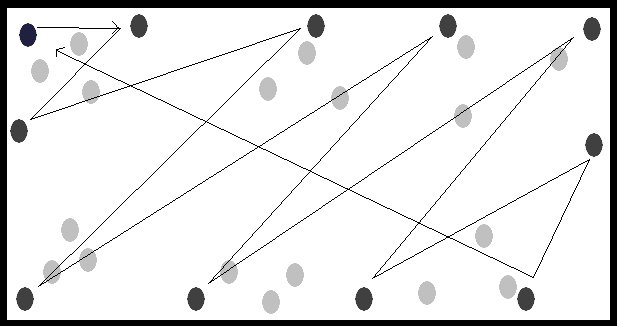
\includegraphics[width=0.9\textwidth]{roaming} % fix pictire
\end{figure}

\subparagraph{Extraction point} 
The extraction point scouting task is used to scout all the metal extraction
points on the map, the scout unit will visit the closest non visited extraction
point until every extraction point has been visited. This task gives us very
valuable information, just like the roaming scout task, but it's much faster to
execute and therefore gives results faster which benefits our priority system. However if the
extraction points aren't scattered in a favorably way this scout task will not explore the whole map
leaving black undiscovered areas.

\paragraph{Attack tasks}
\label{sec:attack_tasks}
Al Ice does not have a complete set of attack tasks. For v0.3 of Al Ice two versions of attacks have
been implemented. A ground attack that attacks ground targets, and an air attack that attacks air
units. Both of these tasks derive from the base attack that is an abstract task class.

\subparagraph{Attack Target}
Attack target is a simple task when assigning a unit to attack a single target. The unit will hunt
down the target as long as it is alive and can be seen by Al Ice. If it's killed it will return a
successful completion whereas it will return an unexpected error when the target escaped from our
line-of-sight.

\subparagraph{Base attack}
\index{base attack}
The abstract task class that 'all' attack tasks derive from. The base attack task needs a set of
attacking units and optional healers if the attack group should have designated healers to it.
However the healers aren't used in the current version, but are implemented as a stub feature.

When the base attack is run it starts off with regrouping all the unit to the group's center
position. If this isn't done the units could be scattered around in the map and would not attack as a mass. As
soon as all units has reached the regroup position it will find a target destination to go to. This
destination if found using the abstract method \texttt{getTargetLocation()} which the derived classes
implements; thus the derived class can find a target destination. E.g. it can be an outpost, flying
unit etc. When the target destination is reached and cleared of enemies it will try to find a new
target destination---this will keep going until all the attacking units are dead.

Whenever an enemy unit is close to the groups center position it will assign attack tasks to attack
the enemy for all attacking units. To get a close enemy it uses the second abstract method
\texttt{getCloseEnemy()} that the derived classes implements; this makes that the derived class has
total control of deciding which enemy to attack. After the enemy has died or escaped the units
returns to their previous task; regroup or move to target destination.

\subparagraph{Ground attack}
\index{ground attack}
The ground attack that derives from base attack has one primary strategy; destroy the enemies metal
extractors if some exists (if we have seen one lately). If it can't find any metal extractors it will
target the nearest enemy ground unit. The \texttt{getCloseEnemy()} simply returns the closest
enemy ground unit to the group's center position that is inside a certain radius. The task takes a
set of attackers as input parameters and optional healers, which is what the base attack task needs. The
General\index{General} decides how large the attack force should be.

\subparagraph{Air attack}
The air attack only attacks air targets, being that air units are in minority of the units the
number of air attacks will probably not be high if the enemy doesn't use a huge amount of air units.
\texttt{getTargetLocation()} returns the last seen position of an air unit and
\texttt{getCloseEnemy} returns the closest enemy air unit that is inside the range specified by a
status. As with the ground attack task it needs an attack force and the General decides how large
the attack force should be.
